\chapter{Introduction} \label{ch:intro}
Consider some typical mathematics problems that you've seen so far in your mathematics education. For example, an algebra exercise
\begin{align}
2x = x + 1 \quad \implies \quad x=1,
\end{align}
or to find the coordinates of the intersection of two lines
\[
	\left.
	\begin{aligned}
	y &= x+1 \\
	y &= 2x
	\end{aligned}
	\right\}
	\quad \implies 	\quad
	\begin{aligned}
	x=1 \\
	y=2
	\end{aligned}
\]
(I hope you noticed this was just a re-interpretation of the previous question). These two problems had solutions that were numbers, but we can have problems with solutions that are functions. For example the differential equations
\begin{align}
& \frac{dy}{dx} = y \quad \implies \quad y(x) = A e^x, \\
& \frac{d^2y}{dx^2} - 2 \frac{dy}{dx} + 2y = 0 \quad \implies \quad y(x) = e^x \left( A \cos 2x + B \sin 2x\right),
\end{align}
which are in fact families of functions as solutions, for any constants $A$ and $B$. Another familiar example is the solution of the quadratic equation
\begin{align}
\alpha x^2 + \beta x + \gamma \quad \implies \quad x = \frac{-\beta \pm \sqrt{\beta^2 - 4\alpha\gamma}}{2\alpha}.
\end{align}
All these previous examples have solutions that are in some sense simple. They are simple in that they have ``closed form'' solutions, meaning that you can write the solution as explicit numbers, constants representing abritrary numbers, functions like logs, exponentials, trigonometric functions, or as square roots. Such ``simple'' solutions are called \textit{analytic} solutions. Now consider the following theorem:

\theorem{ABEL-RUFFINI~}{}{There is no solution ``in radicals'' for general 5th order or higher polynomials with arbitrary coefficients.}

This theorem is also called ``Abel's impossibility theorem'' for good reason. A solution ``in radicals'' means a formula with $n$th roots in it, like the quadratic formula. Evariste Galois\footnote{Evariste Galois (1811-1832), born in Bourg-la-Reine, laid the foundations of group theory, a hugely important topic in abstract algebra with applications in quantum physics. He died at 21 years old in a duel.} found the simplest polynomial equation with no closed form expression:
\begin{align*}
x^5 - x - 1 = 0.
\end{align*}

\exemple{\upline}{
\begin{figure}[h]
	\begin{center}
	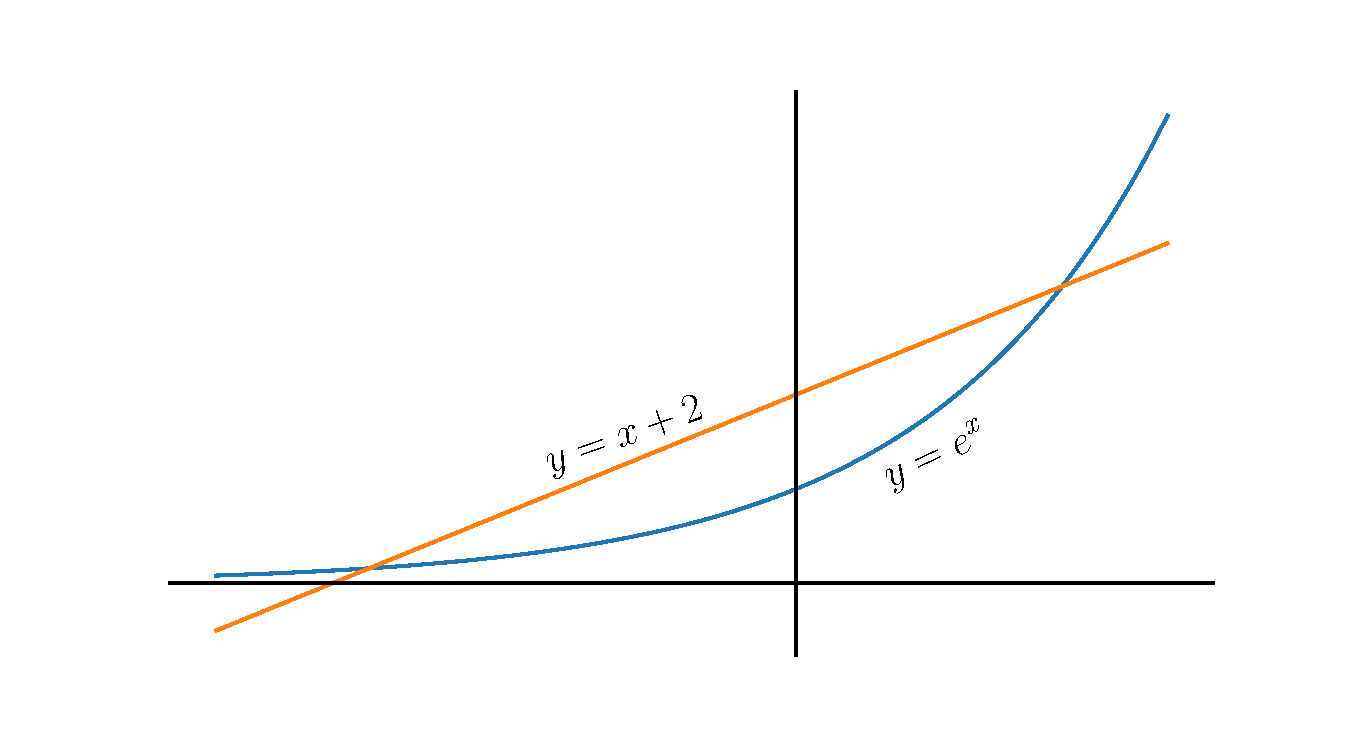
\includegraphics[width=14cm]{figures/intro_intersection.pdf} 
	  \caption{Two points of intersection.} \label{fig:intro_intersection}
	\end{center}
\end{figure}

The simple equation $e^x = x+2$ has no analytic solution. You cannot rearrange it algebraically to end up with $x=\dots$ for some closed form expression. However, it obviously has a solution (in fact 2). The solution is the intersection of two lines
\begin{align*}
y &= e^x, \quad {\rm and} \\
y &= x + 2.
\end{align*}
A simple sketch of these two lines, figure~\ref{fig:intro_intersection}, shows that the two lines must cross at 2 locations. The point is that despite having no \textit{analytic} solution, we will learn \textit{numerical} methods to solving problems like this.}{\downline}



\section{Square root of 2}
How do you know $\sqrt{2} = 1.41421356\dots$? It turns out there are many methods for finding its decimal expansion. We'll look at a few of these methods now to illustrate some basic principles of numerical analysis.


%\subsection{Taylor expansion}
%
%The Taylor\footnote{Brook Taylor (1685-1731), born in Edmonton, England. I don't know anything about this guy.} series of any infinitely differentiable function $f(x)$ at a point $a$ is given by
%\begin{align}
%f(x) = f(a) + f'(a)(x-a) + \frac{f''(a)}{2}(x-a)^2 + \cdots = \sum_{k=0}^{\infty} \frac{f^{(k)}(a)}{k!} \left( x - a \right)^k.
%\end{align}
%To use this for finding $\sqrt{2}$ we define a function
%\begin{align}
%f(x) = (1 + x)^p.
%\end{align}
%We will determine the Taylor series of this function, and then set $x=1$ and $p=1/2$ to have an infinite series giving $\sqrt{2}$. So, we consider successive derivatives
%\begin{align}
%f'(x) &= p(1 + x)^{p-1} \\
%f''(x) &= p(p-1)(1 + x)^{p-2} \\
%f^{(3)}(x) &= p(p-1)(p-2)(1 + x)^{p-3} \\
%f^{(4)}(x) &= p(p-1)(p-2)(p-3)(1 + x)^{p-4} \\
%\vdots \\
%f^{(k)}(x) &= \frac{p!}{(p-k)!}(1 + x)^{p-k}.
%\end{align}
%So we have the Taylor series, choosing $a=0$, of this function
%\begin{align}
%(1 + x)^p = \sum_{k=0}^{\infty} \frac{p!}{k!(p-k)!} x^k = 1 + px + \frac{p(p-1)}{2}x^2 + \frac{p(p-1)(p-2)}{3!}x^3 + \cdots.
%\end{align}
%We can now use this to estimate $\sqrt{2}$ with increasing accuracy as we use more terms
%\begin{align}
%\sqrt{2} = 1 + \frac{1}{2} + \frac{\frac{1}{2}(\frac{1}{2}-1)}{2} + \frac{\frac{1}{2}(\frac{1}{2}-1)(\frac{1}{2}-2)}{3!}  + \frac{\frac{1}{2}(\frac{1}{2}-1)(\frac{1}{2}-2)(\frac{1}{2}-3)}{4!}  + \cdots.
%\end{align}
%In Table~\ref{tab:taylor_sqrt2} the estimate is shown including up to 10 terms. It's quite a slow method, requiring 63 terms before it is stably correct to 3 decimal places.



\subsection{Heron's method}
This method in fact works for computing the square root of any number. Say you want $\sqrt{N}$. Take a first guess $x_0 < N$. This guess could be bigger or smaller than $\sqrt{N}$. If it's smaller
\begin{align}
x_0 < \sqrt{N} \quad & \implies \quad \frac{1}{x_0} > \frac{1}{\sqrt{N}} \\
& \implies \quad \frac{N}{x_0} > \sqrt{N}
\end{align}
Similarly
\begin{align}
x_0 > \sqrt{N} \quad & \implies \quad \frac{N}{x_0} < \sqrt{N}.
\end{align}
In both cases the number we want, $\sqrt{N}$, is between $x_0$ and $\frac{N}{x_0}$. So let's take the next guess as the average of these two
\begin{align}
x_1 = {\rm average}(x_0, \frac{N}{x_0}).
\end{align}
This guess will constrain $\sqrt{N}$ into a smaller interval between $x_1$ and $\frac{N}{x_1}$. So we repeat this procedure as much as we want to converge on $\sqrt{N}$. So we have an iterative scheme for finding the square root of any number, $N$,
\begin{align}
x_{i+1} = \frac{x_i + N/x_i}{2} = \frac{x_i}{2} + \frac{N}{2x_i}.
\end{align}

In the next chapter we will look at \textit{fixed-point analysis}, which studies when iterative schemes stabilise (or not) on fixed points. For example, consider the iterative scheme we just defined for $N=2$, and set the new iterate to be equal to the previous iterate:
\begin{align}
x_i = \frac{x_i}{2} + \frac{1}{x_i}.
\end{align}
Rearranging we see
\begin{align}
x_i - \frac{x_i}{2} = \frac{1}{x_i} \\
\frac{x_i}{2} = \frac{1}{x_i} \\
x_i^2 = 2\\
x_i = \sqrt{2}
\end{align}
Note that this does not mean the scheme will converge on $\sqrt{2}$. It means that if we happen to land on $\sqrt{2}$ on any iteration, then the scheme will stay there.




\subsection{Theon of Smyrna's method}
In this method, we develop an iteration scheme that converges on $\sqrt{2}$. This scheme is given by a ratio

\[
	\begin{aligned}
	x_i = \frac{p_i}{q_i}
	\end{aligned}
	\quad {\rm with} \quad
	\begin{aligned}
	p_{i+1} &= p_i + 2 q_i \\
	q_{i+1} &= p_i + q_i
	\end{aligned}
	\quad {\rm and}  \quad
	\begin{aligned}
	p_0 &= q_0 = 1.
	\end{aligned}
\]
This method only works for computing $\sqrt{2}$


\subsection{Comparison of the methods}


\begin{table}[H]
\begin{center}
\begin{tabular}{c l l}
Iteration & Theon & Heron \\ \hline
0 & 1.00000 & 1.00000 \\
1 & 1.50000 & 1.50000 \\
2 & 1.40000 & 1.41667 \\
3 & 1.41667 & 1.41422 \\
4 & 1.41379 & 1.41421 \\
5 & 1.41429 & 1.41421 \\
6 & 1.41420 & 1.41421 \\
7 & 1.41422 & 1.41421 \\
8 & 1.41421 & 1.41421 \\
9 & 1.41421 & 1.41421 \\
\end{tabular}
\end{center}
\caption{Estimates of $\sqrt{2}$ for the 2 methods.}
\label{tab:taylor_sqrt2}
\end{table}

In the next chapter we will develop other more general methods, based on approximating the solution to the equation
\begin{align*}
x^2 - 2 = 0
\end{align*}
with iterative methods that converge on the exact solution. This clearly the $\sqrt{2}$ that we want to approximate.

%
%\begin{table}[H]
%\begin{center}
%\begin{tabular}{c l l l}
%Iteration & Taylor & Theon & Heron \\ \hline
%0 & 1.00000 & 1.00000 & 1.00000 \\
%1 & 1.50000 & 1.50000 & 1.50000 \\
%2 & 1.37500 & 1.40000 & 1.41667 \\
%3 & 1.43750 & 1.41667 & 1.41422 \\
%4 & 1.39844 & 1.41379 & 1.41421 \\
%5 & 1.42578 & 1.41429 & 1.41421 \\
%6 & 1.40527 & 1.41420 & 1.41421 \\
%7 & 1.42139 & 1.41422 & 1.41421 \\
%8 & 1.40829 & 1.41421 & 1.41421 \\
%9 & 1.41920 & 1.41421 & 1.41421 \\
%\end{tabular}
%\end{center}
%\caption{Estimates of $\sqrt{2}$ for 3 methods.}
%\label{tab:taylor_sqrt2}
%\end{table}




%\section{Order of convergence}



%%%%%%%%%%%%%%%%%%%%%%%%%%%%
%%%%%%%%%%%%%%%%%%%%%%%%%%%%
%%%%%%%%%%%%%%%%%%%%%%%%%%%%
%%%% Exercises %%%%
%%%%%%%%%%%%%%%%%%%%%%%%%%%%
%%%%%%%%%%%%%%%%%%%%%%%%%%%%
%%%%%%%%%%%%%%%%%%%%%%%%%%%%
\exercises{
\section{Exercises}

\exercice{Calculation of $\sqrt{7}$}
%\begin{enumerate}
\begin{enumerate}[label=\alph*)]
	\item Define the function $f(x)$ so that the solution of $f(x)=0$ is $x=\sqrt{7}$. Is there a root of this equation in the interval $[1,2]$? What about $[2,3]$?
	
	\item Use 3 iterations of the bisection method, starting with the interval $[2,3]$, to estimate the value of $x=\sqrt{7}$.
	
	\item How many iterations of the bisection method are required to achieve an accuracy better than $10^{-5}$?
	
	\item Use 3 iterations of Heron’s method, starting at $x_0=3$, to estimate the value of $x=\sqrt{7}$.
\end{enumerate}


\exercice{Calculation of $\sqrt{5}$}
\begin{enumerate}[label=\alph*)]
	\item Give the terms of the Taylor expansion of $(1+x)^p$ for $x=4$ and $p=1/2$ up to the third derivative. Will this series converge on $\sqrt{5}$?
	
	\item Use 3 iterations of Heron’s method, starting at $x_0=2$, to estimate the value of $\sqrt{5}$.
\end{enumerate}


\exercice{Algorithm analysis}
\begin{enumerate}[label=\alph*)]
	\item For Theon of Smyrna’s method, by considering $p^2_{k+1} - 2q^2_{k+1}$ and $p_0=q_0=1$, prove this method converges to $x_0=2$.
	\item Prove that Heron’s method converges for any square root.
\end{enumerate}

}